\section{Durchführung}
\label{sec:Durchführung}
\subsection{Erzeugung der Isotope}
\label{sec:Erzeugung}
Zu Beginn müssen die Isotope Vanadium-52 und Rhodium-104 und -104i durch den Beschuss von Neutronen nach
Kapitel \ref{sec:Neutronenbeschuss} erzeugt werden. Dafür werden die zylindrischen Proben aus Vanadium-51
und Rhodium-103 mit Neutronen aktiviert. 
\subsection{Messung der Strahlung}
\label{sec:Messung}
Die nun Radioaktiven Proben werden dann in die Messapparatur gegeben. Diese ist in Abbildung 
\ref{fig:Apparatur} dargestellt.\\
Die Apparatur besteht dabei aus einem Geiger-Müller-Zählrohr, welches die einfallende Strahlung in 
elektrische Impulse übersetzt. Dieser wird durch einen Verstärker zu einem der beiden Zähler geleitet, 
sodass die Zählrate auf diesem erscheint und abgelesen werden kann. Um die Zählrate in einem bestimmten
Zeitintervall $\Delta t$ durchzuführen, wechselt ein Zeitgeber immer nach der eingestellten Zeit den 
Zähler, sodass immer abwechselnd von den beiden Zählern abgelesen werden kann.\\
Um Störeffekte zu minimieren, ist die Probe mit dem Geiger-Müller-Zählrohr durch einen Bleihülle 
abgeschrimt. Dadurch wird weniger der natürlich vorkommenden Strahlung der Umgebung von dem Zählrohr 
registriert. Dennoch wird auch eine Messung ohne eine Probe durchgeführt, um das Ausmaß der 
Höhenstrahlung und der Strahlung der in der Umgebung vorkommenden radioaktiven Substanzen festzustellen
und in der Berechnung mit einzubeziehen. Dieser Störeffekt wird als Nulleffekt $N_u$ bezeichnet.
\begin{figure}[H]
    \centering
    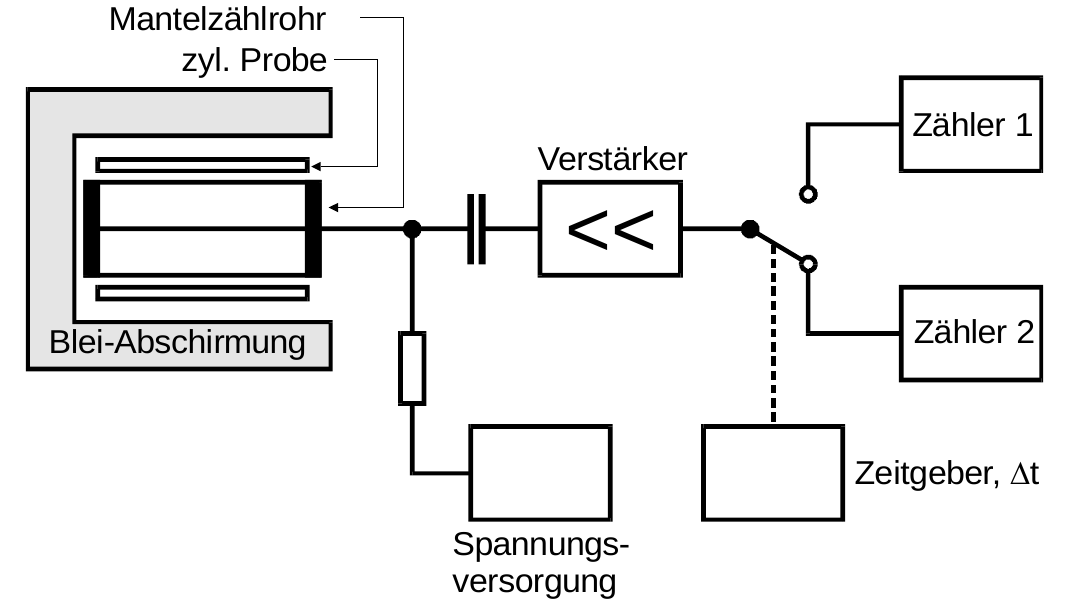
\includegraphics[scale=0.5]{content/Messapparatur.png}
    \caption{Skizze des Versuchsaufbaus. Quelle:\cite{AP01}}
    \label{fig:Apparatur}
  \end{figure}
\noindent Es werden also Folgende Messungen durchgeführt:
\begin{itemize}
    \item $N_u$\\
    In einem Messintervall von $\Delta t=\SI{300}{\second}$ wird ohne eine Probe eine Messung 
    durchgeführt, um den Nulleffekt zu bestimmen.
    \item $N_{V}$\\
    Die Vanadiumprobe wird direkt nach der Aktivierung mit Neutronen in die Messapparatur gegeben. Dann 
    wird in einem Intervall von $\Delta t=\SI{30}{\second}$ die Zählrate notiert 
    \item $N_{Rh}$\\
    Auch die Rhodiumprobe wird direkt nach Aktivierung in die Messapparatur gegeben. Die Zählrate wird 
    nun in einem Intervall von $\Delta t=\SI{15}{\second}$ notiert.
\end{itemize}